\section{Translator}\label{sec:translator}

We develop a dedicated translator to convert \conesc code to plain
nesC. To do so, our translator performs two passes through the input
code. First, it reads the main \code{Makefile} to determine the main
configuration component and to recursively scan the component
tree. Based on the information gained during the first pass, including
the list of every context and context groups defined in the code, it
parses every input file to convert the \conesc code to plain nesC and
to generate a set of support files and additional functionality. The
resulting sources are then compiled using the standard nesC toolchain
to produce a deployment-ready binary.

\putfigure{caption=\conesc translation to nesC code for a generic \code{FooG} context group and an individual context \code{CA}.,label=fig:ctd}{
 \centering
 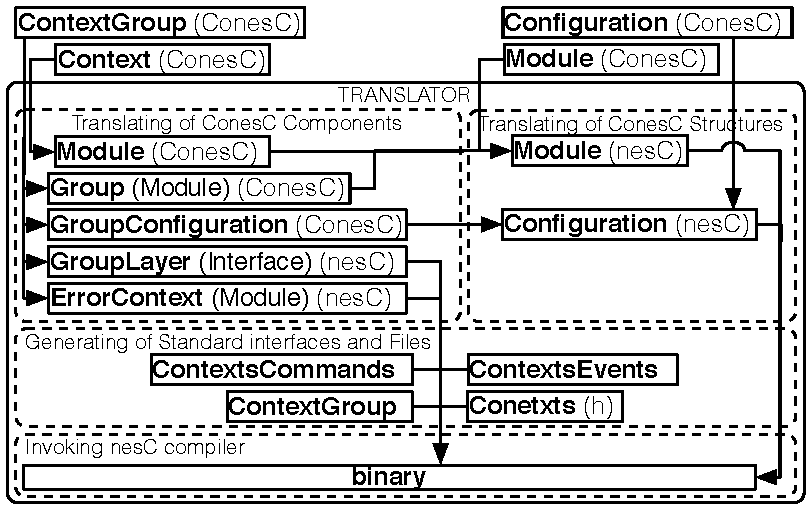
\includegraphics[width=\columnwidth]{pdf/translator}
}

Fig.~\ref{fig:ctd} graphically details the operations during the
second pass. Generally, the input to the translator includes four types
of components: \conesc context groups and contexts, as well as nesC
configurations and modules where some \conesc constructs appear
nonetheless.  In Fig.~\ref{fig:ctd}, context groups and contexts are
presented by a sample \code{FooConG} context group and an individual
\code{FooCon} context therein, whereas nesC configurations and modules with
\conesc constructs are represented as \code{BarC} and \code{BarP},
respectively.

Each context group translates into a custom module that includes the
functionality to implement the dynamic binding of layered functions to
the active context, such as \code{FooConGGroup} in
Fig.~\ref{fig:ctd}. This module is part of a configuration also
automatically generated, such as \code{FooConGGroup} in
Fig.~\ref{fig:ctd}, that in turn implements an automatically generated
nesC interface that exports the layered functions defined in the
group, such as \code{FooConG} in Fig.~\ref{fig:ctd}. Optionally, an
error context is also generated in plain nesC, as indicated by
\code{ErrorFooConGContext} in this case, if the programmer does not
provide one. Each individual context is also translated to a
corresponding nesC module with the proper interfaces to be wired
within the aforementioned configuration, as in the case of
\code{FooConGContext} for the \code{FooConGConfiguration}
Fig.~\ref{fig:ctd}.

At this stage, context and context groups disappeared, yet \conesc
constructs, such as \code{activate} may still appear within the source
code. Our translator converts these constructs to
functionally-equivalent nesC code both in the nesC files generated out
of context groups and individual contexts and in the plain nesC files
that possibly includes them, such as \code{BarC} and \code{BarP} in
Fig.~\ref{fig:ctd}. The resulting sources are then wired to generic
interfaces that define the predefined commands and events in \conesc,
such as \code{contextChanged} for context groups, as in
Fig.~\ref{fig:mm}, and \code{activated/deactivated} for individual
contexts, as in Fig.~\ref{fig:irc} and~\ref{fig:cc}. The result is
plain nesC code that can be given as input to the standard nesC
toolchain.

% \putfigure{caption=Hierarchy of generated components.,label=fig:gfh}{
%  \centering
%  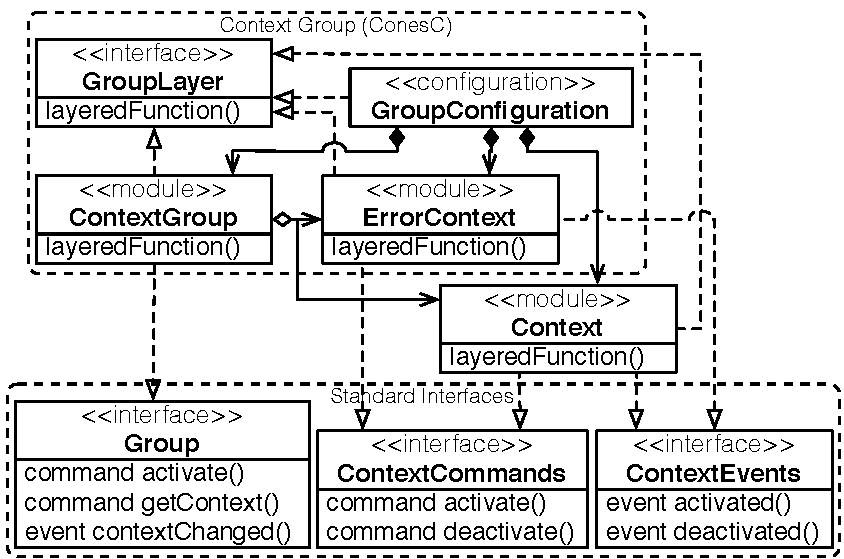
\includegraphics[width=\columnwidth]{pdf/architecture}
% }

% The hierarchy of generated based on \emph{context group} components is displayed
% in Fig.~\ref{fig:gfh}. \emph{GroupLayer} -- a basic interface for all generated
% components -- declares a \emph{layered function}. \emph{GroupConfiguration} is a
% main component, which instantiates \emph{ConetxtGroup} and declared
% \emph{contexts}, and glue them together. The former implements all the internal
% logic to operate by \emph{contexts} and enable behavioral variation.
% \emph{ErrorContext} module is generated if it was not declared in the
% \emph{context group}. \emph{Context} is translated into module by adding
% standard functions and implementation of \emph{group layer} interface mentioned
% above.

% The generated components and written by a developer modules are translated then
% from \conesc into nesC. After that the translator generates standard interfaces
% for additional functionality -- e.g. activation and deactivation of contexts --
% for \emph{ContextGroup} and \emph{contexts}. \emph{Contexts.h} is a definition
% of all the contexts in the projects. The last step is invoking the nesC compiler
% to build a binary by using all the generated and transformed components.

Our translator is implemented in Java using JavaCC~\cite{javacc} for
parsing. Two aspects are worth noticing in its operation. First, the
generated code is completely hardware-independent. Therefore, hardware
compatibility is the same as the original nesC toolchain, allowing us
to support a wide range of WSN platforms and not to modify our
translator due to hardware idiosyncrasies. Second, the whole
translation process is only seemingly straightforward. Rendering the
logic embedded within the \conesc abstractions does require a fairly
sophisticated processing. To give an intuition, we measured the size
of the \conesc implementations of the application we use for
evaluation, described next, against the size of the nesC
implementations output by our translator. On average, we observe three
times as much lines of code in the latter compared to the former.

%%% Local Variables: 
%%% mode: latex
%%% TeX-master: "bare_conf"
%%% End: 
